\section{FUNDAMENTAÇÃO TEÓRICA}

A seguir, serão detalhados os principais conceitos envolvidos e utilizados durante este trabalho.

\begin{comment}
\subsection{Mineração de dados}

De acordo com \citeonline{tan2009DataMining} é o processo de descoberta automática de informações uteis em grandes repositórios de dados. Técnicas de mineração de dados são utilizadas em grandes bancos de dados a fim de descobrir padrões que até então, seriam desconhecidos. Essas técnicas quando aplicadas 
%precisa de mais referências (?)
\end{comment}

%Mineração de textos
\subsection{Mineração de Textos}
Mineração de Texto ou \textit{Text Mining} é definido como uma técnica de análise e extração de conhecimentos a partir de textos, frases ou palavras, com o objetivo de identificar informações úteis e implícitas contidas nos dados armazenados em formato não estruturado. Envolve a aplicação de algoritmos computacionais que processam textos e identificam as informações úteis e implícitas, que normalmente não poderiam ser recuperadas utilizando métodos tradicionais de consulta, pois a informação contida nestes textos não pode ser obtida de forma direta. \cite{morais2007mineraccao}.

Dados em formato não estruturado representam uma grande quantidade de informações nos mais variados ambientes. Esses dados são constituídos de informações que não estão presentes em bancos de dados organizados, mas sim em e-mails, cartas, contratos, e até mesmo comentários da internet. Por serem escritos por humanos para leitores humanos, e não são acessíveis diretamente para computadores, precisam de processamento de Linguagem Natural (NLP), para que tenham sua informação extraída \cite{Dorre1999TMFTextMining}. \citeonline{lucasAraujo2015} Afirma que a prática de mineração de textos pode ser realizada em qualquer domínio que utiliza-se de textos, normalmente contidos em documentos, aplicando-se algoritmos computacionais para processar os textos e conseguir obter conhecimento contido no formato de dados não estruturados. 

De forma geral as etapas da mineração de texto são: seleção de documentos, definição do tipo de abordagem dos dados (análise semântica ou estatística), preparação dos dados, indexação e normalização, cálculo da relevâncias dos termos, seleção dos termos e pós-processamento (análise dos resultados), como mostrado na Figura \ref{fig:figura-2} \cite{morais2007mineraccao}.

\begin{figure}[H] %use h para forçar que a figura fique abaixo do texto
	\caption{\label{fig:figura-2} Etapas do Processo de Mineração de Texto}
	\begin{center}
	    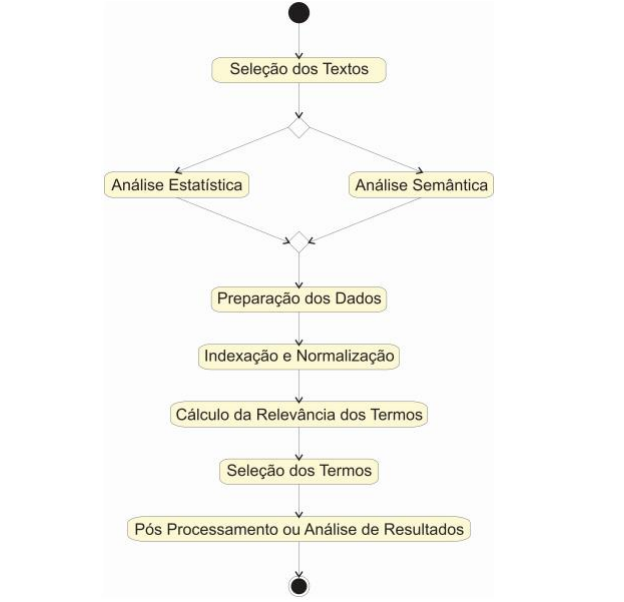
\includegraphics[scale=0.8]{figuras/figura_2.PNG} % altere o atributo scale para o tamanho da figura
	\end{center}
	\legend{Fonte: \citeonline{morais2007mineraccao}}
\end{figure}

\subsubsection{Abordagem dos dados}
\citeonline{morais2007mineraccao} apresenta dois tipos de abordagem dos dados textuais na área de mineração de textos: Análise Semântica, baseada na funcionalidade dos termos encontrados no texto, e Análise Estatística, baseada na frequência dos termos encontrados no texto. Estas abordagens podem ser utilizadas de forma separada ou em conjunto. A abordagem utilizada neste trabalho é a Análise Semântica.
\subsubsubsection{Análise Semântica}
Análise que avalia a sequência dos termos no texto sendo analisado, para identificar sua função, fundamentada em técnicas de Processamento de Linguagem Natural. A utilização de Análise Semântica se dá pela melhoria na qualidade dos resultados do processo de mineração de textos \cite{morais2007mineraccao}.

\subsubsection{Preparação dos dados}
A preparação dos dados envolve a seleção de dados que constituem a base de textos de interesse e o trabalho inicial para tentar selecionar o núcleo que melhor expressa o conteúdo desses textos. Além de prover uma redução dimensional, esta etapa procura identificar similaridades em função da morfologia ou do significado dos termos nos textos \cite{morais2007mineraccao}.

\subsubsection{Indexação e Normalização}
O objetivo principal da indexação e normalização dos textos é facilitar a identificação de similaridade de significado entre suas palavras, considerando variações morfológicas e problemas de sinonímia \cite{morais2007mineraccao}. Este processo tem como resultado a geração de um índice, construído através de um processo de indexação. Um documento pode ser indexado por termos diferentes que são correspondentes ao vocabulário utilizado em sua área. Nesse caso, geralmente, há um conjunto de termos predefinidos e específicos para cada assunto da área em questão \citeonline{morais2007mineraccao}.

Em mineração de textos, a indexação é um processo automático. Suas principais fases são: \textit{identificação de termos} (simples ou composto); remoção de \textit{stopwords} (palavras irrelevantes); e \textit{normalização morfológica} (stemming) \cite{morais2007mineraccao}.

\begin{figure}[H] %use h para forçar que a figura fique abaixo do texto
	\caption{\label{fig:figura-4} Etapas do Processo de Indexação Automática}
	\begin{center}
	    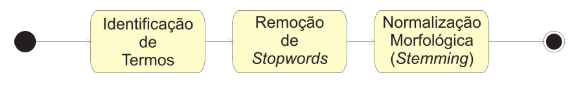
\includegraphics[scale=0.8]{figuras/figura_4.PNG} % altere o atributo scale para o tamanho da figura
	\end{center}
	\legend{Fonte: \citeonline{morais2007mineraccao}}
\end{figure}

\subsubsection{Cálculo de relevância dos termos}
Com exceção das \textit{stopwords}, os termos mais frequentemente utilizados no texto, costumam ter maior importância, assim como palavras constantes em títulos ou em outras estruturas, uma vez que foram colocadas ali por serem consideradas relevantes para a idéia do documento \cite{morais2007mineraccao}.

O cálculo de relevância de uma palavra em relação ao texto que está inserida pode se basear na frequência da mesma, na análise estrutural do documento, ou na posição sintática da palavra. Ao grau de relacionamento da palavra com o texto dá-se o nome de \textit{peso}. Logo é o peso que indica a importância da palavra em relação ao texto \cite{morais2007mineraccao}. 

Existem várias formas de cálculo do peso, as mais comum são baseadas em cálculos simples de frequência: \textit{frequência absoluta, frequência relativa, frequência inversa de documentos.}

\subsubsection{Seleção dos termos}
Seleção de termos corresponde à etapa de seleção das palavras retiradas do texto, após os
processos de pré-processamento e cálculo da relevância. Esta técnica pode ser baseada no peso dos termos ou na sua posição sintática em relação ao texto \cite{morais2007mineraccao}.

É possível aplicar as técnicas de análise sintática e semântica para identificar as palavras mais importantes de um documento. A análise sintática pode ser realizada a partir de um  dicionário ou gramática bem definida para um domínio específico. A análise semântica baseia-se no princípio de que partes mais relevantes de um documento já estão de alguma forma demarcadas por estruturas de formatação específicas para isso.

\subsubsection{Pós processamento ou análise dos resultados}
Esta fase envolve a aplicação de técnicas de análise dos resultados de um Sistema de Recuperação de Informações de Texto, particularmente os resultados do processo de mineração de textos \cite{morais2007mineraccao}.
\citeonline{morais2007mineraccao} ainda afirma que a análise pode ser utilizada como forma de avaliação do Sistema de Recuperações de Informação de Texto, para saber se funcionou como deveria ou não.

\begin{comment}
Neste sentido, a área de Recuperação de Informação (RI) desenvolveu modelos para a
representação de grandes coleções de textos que identificam documentos sobre tópicos específicos. Segundo Ebecken et al. [5], pode-se considerar que a RI seja o primeiro passo de um processo de preparação dos dados.
%Checar!
\end{comment}

\subsection{Processamento de Linguagem Natural}
\citeonline{liddy2001naturallanguage} define \textit{Processamento de Linguagem Natural (Natural Language Processing - NLP)} como um conjunto de técnicas para analisar e representar textos de origem natural, em um ou mais níveis de análise linguística com o propósito de atingir processamento linguístico similar ao humano para um conjunto de tarefas ou aplicações. 

Para mineração de textos armazenados em formato não estruturados, são necessárias técnicas e ferramentas específicas da área de \textit{Descoberta de Conhecimento em Textos (Knowledge Discovery from Text - KDT)} \cite{morais2007mineraccao}. Para recuperação de informação, KDT e mineração de textos possuem alto grau de dependência de Processamento de Linguagem Natural.

Neste trabalho, NLP é utilizada tendo em vista que o ato de interpretar e manipular palavras como parte de uma linguagem é considerado Processamento de Linguagem Natural \cite{morais2007mineraccao}.


\subsection{SentiStrength}
SentiStrength é um classificador léxico que utiliza regras de linguística para detectar a força de um sentimento em uma frase \cite{thelwall2012sentistrength}.

Para cada texto classificado, a ferramenta gera dois valores inteiros que variam de 1 a 5 numa escala positiva e 1 a 5 numa escala negativa, sendo o valor 1, um indicador de neutralidade para o sentimento. Por exemplo, uma classificação que retorna 3, 5 indica uma nota 3 para o sentimento positivo e nota 5 para o sentimento negativo, nesse caso o texto tem mais força negativa do que positiva \cite{thelwall2012sentistrength}.

Originalmente o classificador SentiStrength apenas trabalha com frases no idioma inglês, porém é possível adaptar seu dicionário para outros idiomas. O dicionário utilizado pelo autor neste trabalho, parte do dicionário português padrão que acompanha o SentiStrength, porém adaptado com mais palavrões e algumas correções, para uma detecção mais abrangente. O dicionário utilizado pode ser encontrado no Apêndice A Tabela \ref{appendix:dicionario-sentistrength}. Além disso, foi feito um script \footnote{https://gist.github.com/ssisaias/08b2c8494a4553612987c9d4ae94f86c} para converter a classificação gerada pela ferramenta, para a entrada esperada pelo classificador Naïve Bayes, essa etapa é descrita na seção de procedimentos.

%preciso melhorar essa definição de bayes.
\subsection{Naive Bayes}
Segundo \citeonline{tan2009DataMining}, uma técnica de classificação é uma maneira de construir modelos de classificação a partir de um \textit{Dataset}. Exemplos de classificadores são: Árvore de decisão; Rede Neurais; SVM (Support Vector Machines); e classificadores Naïve Bayes.
Cada uma dessas técnicas aplica um algoritmo de aprendizagem para identificar o modelo que melhor descreve um relacionamento entre o conjunto de atributos e as classes dos dados de entrada. Sendo assim o modelo gerado pelo algoritmo de aprendizagem deve ser capaz de, a partir de um conjunto de entradas, classificar corretamente registros que não eram conhecidos até então.

Naïve Bayes é um dos algoritmos mais eficientes para \textit{machine learning} e mineração de textos. Esse algoritmo de aprendizagem supervisionado utiliza do Teorema de Bayes, porém considerando haver independência entre as \textit{features} (característica das variáveis de entrada) do conteúdo sendo classificado \cite{zhang2004optimalitybayes}.

De acordo com com \citeonline{zhang2004optimalitybayes}, o Teorema de Bayes com features dependentes pode ser definido da seguinte maneira, onde a probabilidade de um evento $\epsilon$ ser da classe $c$ é:

\begin{equation}
\label{eq:bayes_classic}
 P(c|\epsilon) = P(c ) \frac{P(\epsilon |c)}{P(\epsilon)}
\end{equation}

$\epsilon$ pertence a classe $C = +$ se somente se:
\begin{equation}
\label{eq:bayes_classic}
 {f_b}(\epsilon) =  \frac{P(C = + | \epsilon)}{P(C = - | \epsilon)} \geq 1
\end{equation}

onde ${f_b}(\epsilon)$ é um classificador Bayesiano.

Se assumirmos que os atributos são independentes dados os valores de classe, ou seja:
\begin{equation}
\label{eq:naive_bayes}
 {p}(\epsilon|c) =  {p}({x_1, x_2, ..., x_n}|c) = \prod_{i=1}^{n} {p}(x_i|c),
\end{equation}

O classificador resultante é:

\begin{equation}
\label{eq:bayes_classic}
 {f_nb}(\epsilon) =  \frac{P(C = +)}{P(C = -)} \prod_{i=1}^{n} \frac{P({x_i} | C = +)}{P({x_i} | C = -)}
\end{equation}

A função ${f_nb}(\epsilon)$ é chamada de classificador Naive Bayes (naive Bayesian classifier).

A utização do Naïve Bayes se dara através da ferramenta scikit-learn \citeonline{scikit-learn}, onde o classificador já está previamente implementado.
%% Old content
\begin{comment}

\citeonline{zhang2004optimalitybayes} define o algoritmo Naïve Bayes como um \textit{Teorema de Bayes} com independência condicional entre as variáveis $A_1...A_n$ dada uma categoria $C$. Na figura \ref{fig:figura-bayes}, $C$ é o nó pai e $A_1...A_n$ são nós filhos. Como $A_1...A_n$ são independentes entre si, dado $C$, temos que $P(A_i|C,A_j)=P(A_i|C)$

\begin{figure}[H] %use h para forçar que a figura fique abaixo do texto
	\caption{\label{fig:figura-bayes} Rede Naïve Bayes}
	\begin{center}
	    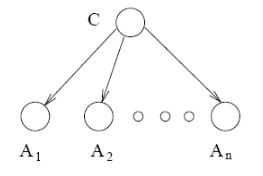
\includegraphics[scale=1]{figuras/figura_5.PNG} % altere o atributo scale para o tamanho da figura
	\end{center}
	\legend{Fonte: \citeonline{ZhangandLi2007Bayes}}
\end{figure}


Numa tarefa de inferência probabilística, o objetivo é calcular a probabilidade de uma hipótese $C$ dado que os dados $A_1...A_n$ fora observados, descrita como $P(C|A_1,...,A_n)$ \cite{ZhangandLi2007Bayes}.
%Tem outras etapas do algoritmo que o tan apresenta em 3.1

\end{comment}